The \texttt{\pkglnk{model.parsing}} package contains the classes necessary to turn an input String into a \texttt{\hyperref[type:edu.kit.wavelength.client.model.term.LambdaTerm]{LambdaTerm}} object.
This process is initiate by the \texttt{\lnk{ExecutionEngine}} instancing a new \texttt{\lnk{Parser}} object with the currently activated \texttt{\hyperref[type:edu.kit.wavelength.client.model.libraray.Library]{Library}} and invoking its parse method. The \texttt{\lnk{Parser}} in turn uses the \texttt{\lnk{Tokeniser}} to turn the input String into a sequence of \texttt{\lnk{Token}}s. 

Each \texttt{\lnk{Token}} contains a section of original input String. This substring is passed to the \texttt{\lnk{Token}} on its creation by the \texttt{\lnk{Tokeniser}} and can be access trough the \texttt{\lnk{Token}}s interface.

From this sequence the \texttt{\lnk{Parser}} builds a \texttt{\hyperref[type:edu.kit.wavelength.client.model.term.LambdaTerm]{LambdaTerm}} object structure.
If the input contains names referencing library terms and the \texttt{\lnk{Parser}} is initialized with the necessary \texttt{\hyperref[type:edu.kit.wavelength.client.model.libraray.Library]{Library}}s, the terms will be incorporated in the \texttt{\hyperref[type:edu.kit.wavelength.client.model.term.LambdaTerm]{LambdaTerm}} object and their names conserved.
 
If the input String can not be parsed a \texttt{\lnk{ParseEception}} is thrown.
The \texttt{\lnk{ParseEception}} contains an error message describing the error which led to its creation, and where in the input String the error occurred.
Both message and location can be accessed and printed to the output window to aid the user in correcting the error.

\begin{figure}[H]
	\centering
	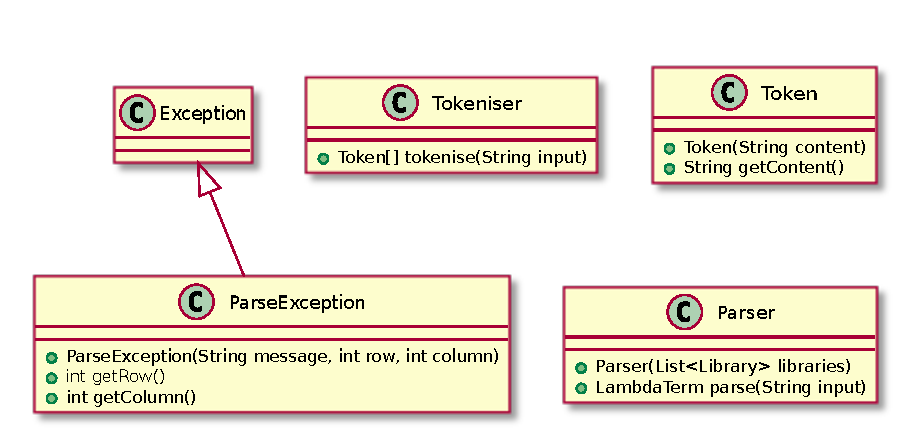
\includegraphics[width=\textwidth]{packageDiagrams/parsingPackage}
\end{figure}
